\section{Fissione e Fusione Nucleare}

\subsection{Fissione Nucleare}
\paragraph{Fissione spontanea}
Perché tutti gli elementi con numero di massa elevato non decadono spontaneamente in $^{56}Fe$?

Quando si è parlato della formula semiempirica di massa, si è visto che una delle logiche di funzionamento della natura è che la somma dei protoni e neutroni legati è minore della somma dei pesi degli elementi slegati. 
La differenza di massa è l'energia di legame
\[
\Delta mc^2=BE.
\]
Essendo che il ferro come abbiamo visto è l'elemento con l'energia di legame maggiore, è lecito chiedersi cosa blocchi un eventuale decadimento dei nuclei più pesanti nel ferro in quanto energeticamente favorevole (massimizzando l'energia di legame minimizzo l'energia di massa).
\[
A\to A/2?
\]
Per passare da uno stato $A$ legato a due nuclei $A/2$ bisogna necessariamente per uno stato intermedio di un nucleo deformato dove sono presenti due nuclei legati tra loro ma identificati.
Studiamo quindi questo stato intermedio 
\begin{equation}
BE= a_v A-a_s A^{2/3}-a_c \frac{Z(Z-1)}{A^{1/3}}-a_{sym}\frac{(N-Z)^2}{A}+\delta_p
\end{equation}
In questo caso ignoriamo quello che è il termine di accoppiamento $\delta_p$ considerando il caso di due nuclei \emph{even-even}.
Vogliamo confrontare l'energia di legame del nucleo unico (1) al caso del nucleo quasi separato (2).

Il termine di volume sarà:
\begin{enumerate}
\item $a_v A$
\item $2a_v \frac{A}{2}$
\end{enumerate}
Questi due termini sono uguali, il che non è sorprendente perché il modello a goccia mantiene costante il volume.

Prendiamo ora il termine di simmetria:
\begin{enumerate}
\item $a_{sym}\frac{(N-Z)^2}{A}$
\item $a_{sym} 2\biggl[\frac{(N/2 -Z/2)^2}{A/2}=a_{sym}\frac{(N-Z)^2}{A}$
\end{enumerate}
Nemmeno questo termine varia.

Consideriamo il termine di superficie:
\begin{equation}
V_1=V_2\to \frac{4}{3}\pi R^3=2\frac{4}{3}\pi r^3
\end{equation}
\begin{equation}
R^3=2r^3\to R=1,26 r
\end{equation}
\begin{enumerate}
\item $S_1=4\pi R^2=4\pi(1,26)^2r^2=6\pi r^2$
\item $S^2=2\cdot 4\pi r^2=8\pi r^2$
\end{enumerate}
Se deformiamo un nucleo la superficie aumenta, il che comporta un aumento del termine di superficie e quindi una diminuzione dell'energia di legame.

Vediamo dunque come si comporta il termine coulombiano:
\begin{enumerate}
\item $V_1=\frac{a_c Z(Z-1)}{A^{1/3}}$
\item $V_2= \frac{2(a_c Z/2 (Z/2-1))}{(a/2)^{1/3}}=\frac{1,26\cdot2}{4}\frac{a_c Z(Z-2)}{a^{1/3}}$
\end{enumerate}
Da un confronto con nuclei ad alto Z, la differenza tra $Z-1$ e $Z-2$ è trascurabile
\begin{equation}
V_2\sim \frac{2}{3} v_1
\end{equation}
In questo caso si ha che il termine coulombiano diminuisce con la formazione dello stato intermedio, il che comporta un aumento dell'energia di legame.

Qual è quindi il termine dominante in questa fase intermedia?

Posso prendere come riferimento i valori che erano stati trovati dei termini
\[
a_c=0,7MeV \hspace{0.2cm}a_s=18MeV
\]
Il termine dominante è quindi il termine di superficie, si ha quindi che nella fase intermedia l'energia di legame diminuirà, portando ad un'energia di massa maggiore, creando così una barriera di potenziale.
Per questo è impossibile una fissione spontanea dei nuclei più pesanti del Ferro.
La $\Delta E\approx 6MeV$ tra il nucleo legato e lo stato intermedio è chiamata \emph{energia di attivazione}.
I nuclei che fanno fissione spontanea sono i nuclei che hanno 
\begin{equation}
\frac{Z^2}{A}>51
\end{equation}

\paragraph{Fissione Indotta}
La differenza energetica evidenziata nel primo paragrafo corrisponde più esattamente a 
\begin{equation}
\Delta E=6,2MeV
\end{equation}
Il processo sfruttato è quello di inviare neutroni su nuclei di Uranio, il primo a effettuare questo processo fu Fermi che però non riconobbe il fenomeno.
\begin{equation}
n+^{235}U\longrightarrow X+Y+Nn+Q
\end{equation}
Il pensiero più logico è quello che in questo processo per superare l'energia di attivazione si debba prendere un neutrone abbastanza energetico che trasferisca l'energia di attivazione necessaria a far cominciare il processo.
\begin{figure}[h]
\centering
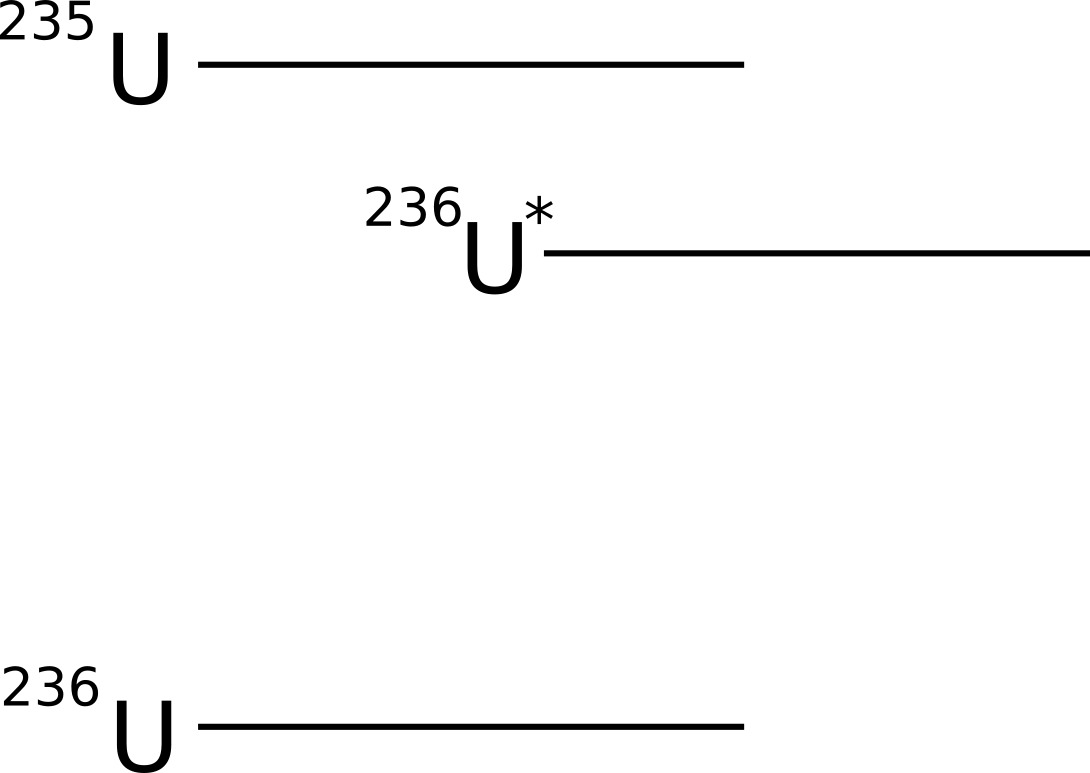
\includegraphics[width=120pt]{fig6_01}
\caption{Livelli che interessano la fissione indotta dell'uranio 235.}
\end{figure}

In realtà si è visto che questo tipo di fenomeno si verifica con neutroni termici (ovvero neutroni a temperatura ambiente) che possiedono quindi energia pari a 
\begin{equation}
E=KT=\SI{9e-5}{\frac{eV}{K}}\times 300K=\SI{27e-3}{eV}
\end{equation}
Un'energia molto minore all'energia di attivazione!

Quello che si verifica è che un neutrone termico assorbito dall'Uranio da origine ad un atomo di Uranio 236 in uno stato eccitato con energia maggiore dell'energia di attivazione.
\begin{equation}
n+^{235}U\to ^{236}_{92}U*
\end{equation}

Da notare che in natura la composizione dell'uranio è
\[
^{238}U\hspace{0.1cm} al\hspace{0.1cm} 99,28\%\hspace{0.5cm}^{235}U\hspace{0.1cm} al\hspace{0.1cm} 0,72\%
\]
E nel caso dell'uranio 238 lo stato che si viene a formare dopo l'assorbimento di un neutrone ha energia pari a $4,8MeV$ che non basta per innescare il decadimento, per processi di fissione nucleare viene quindi sfruttato solamente $^{235}U$.
Dal punto di vista fisico questo si rappresenta tramite la sezione d'urto.

Facendo un grafico della sezione d'urto si ha che questa, partendo da un valore iniziale di $500b$, diminuisce aumentando l'energia.
Questo effetto è dovuto al fatto che aumentando l'energia è vero che si supera più facilmente la barriera di potenziale ma sarà anche più difficile mantenere nel nucleo il neutrone che tenderà invece a fuggire.
\'E quindi conveniente usare i neutroni a più bassa energia disponibili alla fissione.
Il bilancio energetico per cattura neutronica da $^{235}U$ e $^{238}U$ è dovuto al termine di accoppiamento $\delta _q$ nella formula semiempirica di massa, infatti, mentre l'uranio 235 ha un numero dispari di neutroni che comporta una tendenza ad assorbire un neutrone per pareggiare il livello energetico, l'uranio 238 ha un numero pari di entrambi gli elementi che porta ad una stabilità che evita l'assorbimento neutronico spontaneo (non c'è quindi l'energia addizionale di accoppiamento).

Qual è la distribuzione di massa dei prodotti di reazione?
La previsione fatta era che i nuclei si dividessero come:
\[
A\longrightarrow 2A/2
\]
In questo caso la formula semiempirica di massa fa una predizione sbagliata infatti è stato verificato sperimentalmente che per esempio i nuclei di uranio hanno la tendenza a produrre con maggior frequenza nuclei con numeri di massa in distribuzione gaussiana attorno a $A=95,140$ con un minimo centrale tra i due picchi a $A=118$.

In questo caso ciò che subentra è il modello a shell, i nuclei generati tenderanno ad addensarsi attorno ai nuclei che abbiamo visto essere più stabili nel modello a shell nucleonico.
I nuclei figli che si trovano ad avere più neutroni rispetto alle valli di stabilità tenderanno a decadere $\beta^-$ per tornare in uno stato stabile.

Restando in questo argomento dei prodotti di fissione prendiamo un caso particolare:
\begin{equation}
n+^{235}U \longrightarrow ^{236}U*\longrightarrow^{140}_{54}Xe+^{94}_{38}Sr+2n
\end{equation}
I modi di fissione dell'uranio sono vari e un ingegnere di una centrale nucleare deve conoscerli tutti. In questo caso il processo non si ferma lì ma decadono pure i nuclei figli con un processo di decadimento $\beta^-$:
\begin{equation}
\begin{split}
^{140}_{54}Xe &\longrightarrow ^{140}_{55}Cs \longrightarrow ^{140}_{56}Ba \longrightarrow ^{140}_{57}La \longrightarrow ^{140}_{58}Ce\\
^{94}_{38}Sr&\longrightarrow^{94}_{39}Y \longrightarrow^{94}_{40}Zr
\end{split}
\end{equation}
Un altro modo di decadimento è:
\begin{equation}
^{236}U\longrightarrow^{137}_{53}I+^{97}Y+2n+Q
\end{equation}
In questo caso lo Xeon decade come:
\begin{equation}
^{137}_{53}I \longrightarrow^{137}_{54}Xe\longrightarrow^{136}_{54}Xe+n
\end{equation}
Lo Xeon è essenziale per il funzionamento delle centrali nucleari e in particolare quest'ultimo processo che porta all'emissione di neutroni è fondamentale nel controllo del reattore.

Il processo di fissione avviene con un tempo caratteristico di $t=10^{-12}s$.
I neutroni emessi nel processo principale vengono chiamati \emph{neutroni prompt}, quelli che invece vengono generati nei processi di decadimento sono chiamati \emph{neutroni ritardati}.
Quest'ultimi sono ciò che tiene sotto controllo il reattore nucleare e se non ci fossero non saremmo in grado di far funzionare i reattori.
I neutroni prompt sono invece quelli fondamentali alla produzione di energia.

\paragraph{Principi di funzionamento di un reattore nucleare a fissione}
Abbiamo visto che la fissione dell'$^{235}U$ avviene con un processo del tipo
\begin{equation}
n+^{235}U\longrightarrow^{236}U*\longrightarrow X+Y+2n+Q
\end{equation}

Un reattore nucleare è formato da un contenitore che scherma dalle radiazioni emesse dai prodotti di reazione.
All'interno sono poste le barre di combustibile ovvero di materiale reagente.
Per raccogliere il calore il contenitore è pieno di liquido refrigerante, normalmente di acqua, che attraverso delle condutture viene raccolta e convogliata attraverso uno scambiatore di calore che invia poi l'acqua all'interno del reattore.
Il meccanismo di raffreddamento dell'acqua e quindi di produzione energetica è uguale a quello di qualsiasi altra centrale elettrica, ciò che cambia è solamente il metodo di riscaldamento.
 
 Ci sono due tipi di problemi che si presentano all'interno di un reattore:
\begin{enumerate}
\item \textbf{Dobbiamo rallentare i neutroni.} 
I neutroni prodotti nella reazione non sono a energia termica e abbiamo visto che se vogliamo massimizzare la sezione d'urto di cattura dobbiamo diminuire la velocità e portare i neutroni all'energia adeguata.
\item \textbf{Dobbiamo ridurre n a 1.} 
Mediamente il numero di neutroni per fissione è di 2,5 e quindi se non c'è controllo di reazione si ha che ogni 2 reazioni generano in media 5 reazioni. 
Questo non va bene perché porta fuori controllo il reattore che diventa una bomba.
Cerchiamo di avere un rapporto di 1 a 1 tra le reazioni.
\end{enumerate}

Le soluzioni che permettono quindi il corretto funzionamento del reattore sono:
\begin{enumerate}
\item \textbf{Determinazione del moderatore.}
\begin{figure}[h]
\centering
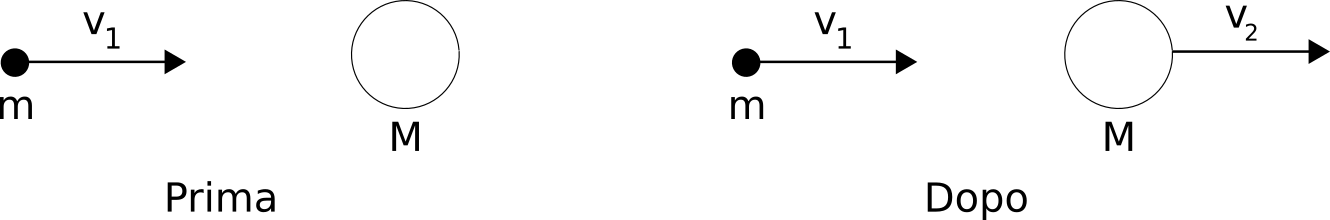
\includegraphics[width=220pt]{fig6_02}
\caption{Interazione di un nucleo con un neutrone}
\end{figure}

Per la conservazione della quantità di moto si ha 
\begin{equation}
\begin{split}
p=cost\hspace{1cm}&mv=mv_1+Mv_2\\
K=cost\hspace{1cm}&\frac{1}{2}mv^2=\frac{1}{2}mv_1^2+\frac{1}{2}Mv_2^2\\
&v_2=\frac{m}{M}(v-v_1)\\
&v_2^2=\frac{m}{M}(v^2-v_1^2)
\end{split}
\end{equation}
Le due formule ottenute sopra possono essere combinate per ottenere 
\begin{equation}
\begin{split}
\frac{m}{M}(v^2-v_2^2)&=\frac{m}{M}(v-v_1)^2\\
Mv^2-Mv_1^2&=m(v-v_1)^2\\
M(v-v_1)(v+v_1)&=m(v-v_1)^2\\
Mv+Mv_1&=mv-mv_1
\end{split}
\end{equation}
Si può quindi ricavare $v_1$ da questa formula ottenendo
\begin{equation}
v_1=v\frac{m-M}{m+M}
\end{equation}
Si può cercare di minimizzare questa velocità per trovare con che materiale si possa termalizzare i neutroni.
La condizione è semplice da vedere:
\[
m\sim M
\]
Il miglior materiale che utilizza il minor numero di urti per rallentare il neutrone è quindi quello che ha massa uguale a quella del neutrone.
Il materiale più utilizzato è l'acqua che presenta caratteristiche termiche ideali, ma soprattutto presenta le caratteristiche ideali per il rallentamento dei neutroni.
L'acqua non è quindi solamente un refrigerante ma anche un moderatore.

\item \textbf{Riduzione dei neutroni prodotti da $N=2,5\to 1$.}

In questo caso possono esserci più modi e in alcuni casi la natura ci viene in contro.
\begin{itemize}
\item Alcuni neutroni vengono assorbiti senza produrre fissione, può accadere infatti che l'Uranio 236 si disecciti tramite emissione $\gamma$.

In questo caso il parametro che ci è utile è $\eta$ che corrisponde alla frazione di neutroni che sopravvive all'assorbimento ($\eta<1$).

\item Il secondo effetto è che alcuni neutroni veloci possono produrre fissione nel Uranio 238 $^{238}U$, infatti anche se nelle centrali viene usato dell'uranio arricchito la percentuale più alta ($97\%$)è di uranio 238.

Per questo effetto teniamo conto di un fattore $\varepsilon$ che corrisponde alla frazione di neutroni prodotti da fissione in $^{238}U$ ($\varepsilon>1$ quindi questi neutroni ne producono comunque altri).

\item Nel grafico della sezione d'urto in funzione dell'energia esiste una regione tra $1\to 100eV$ chiamata \emph{regione delle risonanze}, in cui vengono assorbiti neutroni che vengono eliminati dal ciclo (senza riuscire a termalizzare).

Questo effetto è regolato da $p$ che corrisponde alla frazione di neutroni che sopravvive alle risonanze($p<1$).

\item I neutroni possono essere assorbiti dal moderatore.

Questo viene chiamato fattore $f<1$, in particolare un neutrone può essere assorbito da un protone dell'acqua dando luogo ad un deutone, trasformando quindi l'acqua in quella che viene chiamata acqua pesante.
\[
H_2O\to D_2O
\]
Tra l'altro l'utilizzo dell'acqua pesante come moderatore non ne varia l'efficacia, si abbassa anzi la probabilità che vengano assorbiti neutroni.
Esistono quindi delle centrali che vengono raffreddate e moderate con acqua pesante.
\end{itemize}
Si ha quindi che la frazione di neutroni che sopravvive a questi effetti è dato dalla \emph{formula dei quattro fattori}
\begin{equation}
N=N\eta\varepsilon p f=KN
\end{equation}
introdotta da Fermi.
Per il corretto funzionamento del reattore devo mantenere $K=1$.
\end{enumerate}

\paragraph{Controllo del reattore}
Si abbia
\[
K=1+\delta\hspace{0.5cm}\delta=0,01
\]
I tempi caratteristici della fissione sono $t=10^{-12s}$ che corrisponde al tempo di fissione, seguito poi dal tempo di rallentamento dei neutroni per la generazione di una seconda fissione $t=10^{-3}s=\tau$.

Supponendo che il processo vada avanti per $t$ secondi, il numero di cicli sarà dato da 
\begin{equation}
n=\frac{t}{\tau}
\end{equation}
Dobbiamo considerare che per ogni interazione il numero di neutroni cresce di $1+\delta$.
L'evoluzione dei neutroni è descritta come
\begin{equation}
N(t)=N(0)(1+\delta)^{t/\tau}
\end{equation}
dove $N(x)$ è il numero di neutroni dopo il tempo x, $K=1+\delta$ è il numero di neutroni che si producono ad ogni interazione.
Facendone il logaritmo sin ottiene
\begin{equation}
\ln N(t)=\ln N(0)+\ln(1+\delta)+\frac{t}{\tau}
\end{equation}
Se $\delta$ è piccolo si ha
\begin{equation}
\ln N(t)=\ln N(0)+\frac{t}{\tau}\delta
\end{equation}
Facendo l'esponenziale si trova
\begin{equation}
N(t)=N(0)e^{\frac{t\delta}{\tau}}
\end{equation}
Dopo un tempo $t=1s$ ottengo 
\begin{equation}
N(1)=N(0)e^10
\end{equation}
Si ha quindi un fattore moltiplicativo di $\sim 22026$. E questo descrive un processo controllato il che ci fa comprendere come sia essenziale un controllo efficace di $K$.

Per il controllo  di un reattore oltre al combustibile e al liquido refrigerante bisogna inserire anche delle barre di controllo che assorbono neutroni (per esempio un ottimo materiale di controllo è il cadmio $Cd$).

Un reattore può essere:
\begin{equation}
\begin{split}
&K=1\hspace{1cm}critico\\
&K<1\hspace{1cm}sottocritico\\
&K>1\hspace{1cm}supercritico
\end{split}
\end{equation}
Essendo il tempo di rallentamento dell'ordine del millisecondo, questo non è compatibile con il tempo meccanico di inserimento di queste barre, ma come abbiamo visto il fattore $k$ richiede una precisione estrema perché anche delle piccole variazioni del sistema potrebbero portare ad un collasso rapido.

Per questo vengono in aiuto i \emph{neutroni ritardati}, che vengono sfruttati per portare il reattore a $K=1$ (situazione di criticità).
La reazione che produce i neutroni ritardati come abbiamo visto avviene in un tempo di qualche secondo, questo permette l'inserimento delle barre in un tempo adatto al controllo.

\paragraph{Tipi di Reattori}
\begin{enumerate}
\item \emph{Reattore ad acqua in pressione (PWR).} 
Questo vuol dire che l'acqua all'interno del reattore è sempre nello stato liquido. 
Se infatti portiamo la pressione ad un valore di $100 atm$ allora la temperatura di ebollizione sarà di $300^oC$.
L'acqua viene fatta uscire dal reattore ad una temperatura di $250^oC$ e immessa nello scambiatore dove vaporizza acqua che andrà in forma di vapore ad azionare le turbine come in una qualsiasi altra centrale.
In questo tipo di reattore c'è la necessità di uranio arricchito.

\item \emph{Reattore ad acqua pesante(PHWR).}
In questo caso si usa al posto dell'acqua normale acqua formata con deuterio invece che idrogeno.
Il vantaggio sta nel fatto che per la proprietà di basso assorbimento di neutroni dell'acqua pesante è possibile usare Uranio naturale senza quindi il processo di arricchimento.

\item \emph{Reattore ad acqua bollente(BWR).}
In questo caso l'acqua nel circuito di scambio viene portata ad ebollizione. Si ha che quindi l'acqua del reattore viene portata ad ebollizione.

\item \emph{Reattore con moderatore a grafite.}
In questi reattori viene usata la grafite come moderatore e l'anidride carbonica come refrigerante.
\end{enumerate}

Esistono inoltre altri materiali fissili, infatti tutti i nuclidi della stessa zona dell'uranio con neutroni dispari può innescare una reazione di fissione (per esempio il plutonio 239 $^{239}Pu$ o l'uranio 233 $^{233}U$).
La peculiarità di questo è che l'uranio 238, quando cattura un neutrone, da luogo ad uno stato eccitato dell'uranio 239 che decade in Nettunio 239, che a sua volta decade il plutonio 239.
\begin{equation}
n+ ^{238}U\to ^{239}U*\to ^{239}Np\to ^{239}Pu
\end{equation}
Si ha quindi che alcune catene di reazioni portano da un combustibile ad un altro combustibile.
Un'altra catena possibile è 
\begin{equation}
n+^{232}Th\to ^{233}Th*\to ^{233}Pu\to ^{233}U
\end{equation}

%nuova sezione-------------------------------------------------------------------------
\subsection{Fusione Nucleare}
Prendiamo in considerazione la tabella dell'energia di legame in funzione del numero di massa, come abbiamo già visto il massimo è il ferro 56 che risulta quindi essere il materiale con l'energia di legame più alta.
\begin{figure}[!h]
\centering
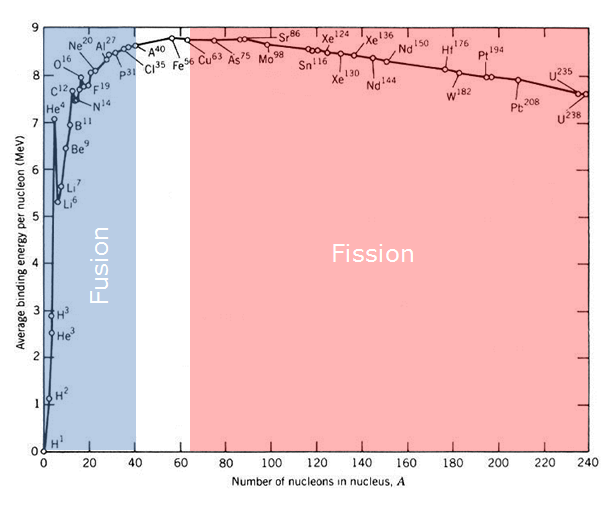
\includegraphics[width=180pt]{fig6_03}
\end{figure}

Come visto nella sezione precedente i materiali pi pesanti del ferro 56, ovvero quelli a destra nel grafico presentano una $\Delta Q$ che rende vantaggiosa la scissione in materiali a numero di massa minore e questo può essere sfruttato per la produzione di energia elettrica nelle centrali nucleari.
Anche nella parte sinistra della curva si ha una $\Delta Q$, con la tendenza inversa rispetto alla fissione, infatti in questo caso i nuclei tenderanno ad ingrandirsi ovvero a legarsi per raggiungere uno stato più legato, sempre con la liberazione di energia.
Dato un elemento X e uno Y il processo di fusione sarà del tipo:
\[
X+Y\longrightarrow Z+\omega+\Delta Q.
\]
Il processo più semplice immaginabile di nucleosintesi è quello tra due protoni
\[
^1_1H+^1_1H\longrightarrow ^2_2He
\]
Come si è visto questo processo però non può avvenire a causa del principio di esclusione di Pauli, è già stato spiegato nel modello di Fermi che è impossibile avere due protoni nello stesso stato quantico (c'è la necessità di almeno un neutrone che abbia spin solidale al protone per poter mettere un protone con spin opposto e riempire lo stato).
In realtà la reazione di fusione di due protoni avviene all'interno del sole e più in generale nelle stelle ma ha un tipo diverso di reazione che avviene grazie all'interazione della forza debole:
\begin{equation}
^1_1H+^1_1H\longrightarrow ^2_1H+e^++\nu_e
\end{equation}

La seconda reazione più semplice che può avvenire è quella di fusione del deuterio
\begin{equation}
^2_1H+^2_1H\longrightarrow ^4_2He+\Delta Q
\end{equation}
Questa è una reazione vantaggiosa sotto più punti di vista.
In primo luogo, si ha che il deuterio, per quanto sia un isotopo e quindi risulti essere molto raro nell'idrogeno, ha comunque una presenza di una particella ogni circa 7000, il che lo rende praticamente illimitato a livello macroscopico facendo comunque parte dell'idrogeno che rimane il materiale più comune in natura.
In secondo luogo, rispetto alla fissione che riguarda materiali molto pesanti che danno origine a prodotti radioattivi, questo processo riguarda materiali leggeri e sia prodotti che reagenti non presentano radioattività.

La difficoltà in tutto questo sta nella difficoltà di fare fondere il deuterio, infatti perché la reazione avvenga bisogna riuscire ad avvicinare i due nuclei di deuterio, superando quella che è la forza di repulsione coulombiana 
\begin{equation}
F=\frac{Z_1Z_2e^2}{4\pi\varepsilon_0 r^2}
\end{equation}
In particolare si ha che questa forza aumenta con il quadrato della distanza mano a mano che si cerca di avvicinare i due nuclei.
\begin{figure}[h]
\centering
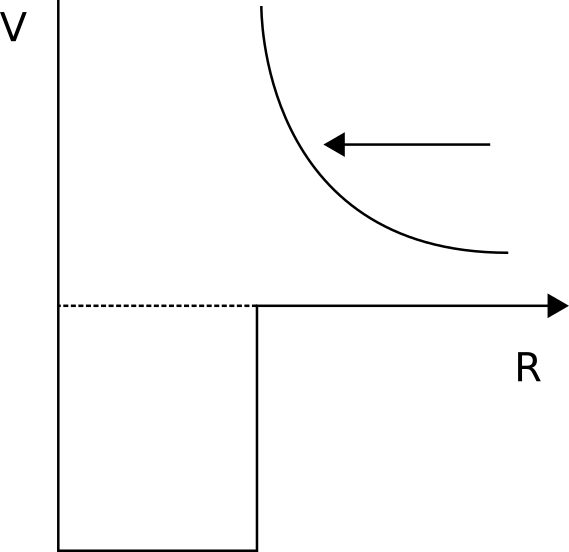
\includegraphics[width=120pt]{fig6_04}
\end{figure}

Rappresentando il potenziale nucleare è vero che se ci si riesce ad avvicinare abbastanza i due deutoni subentra la forza nucleare e i due nuclei sono catturati nella buca, bisogna però considerare che bisogna prima superare la barriera di potenziale data dal potenziale coulombiano. 
La barriera coulombiana avrà un valore di 
\begin{equation}
V_0=\frac{Z_1Z_2e^2}{4\pi\varepsilon_0 R}=\frac{e^2}{4\pi\varepsilon_0 R}\frac{\hbar c}{\hbar c}=\frac{144MeV\cdot fm}{2fm}=0,72MeV=720KeV
\end{equation}
Il valore da raggiungere sarà quindi di $720KeV$ che è un valore facilmente ottenibile in un acceleratore, però in questo caso stiamo parlando di fusione per la produzione di energia, ci serve quindi che il numero di nuclidi che fonde sia elevato e inoltr che l'energia prodotta sia maggiore di quella utilizzata per esempio per far funzionare l'acceleratore.
Dobbiamo basarci quindi sul fatto che la reazione avvenga grazie alla semplice energia termica. 
Il valore energetico a temperatura ambiente è
\begin{equation}
E=KT=\SI{9e-9}{\frac{eV}{K}}300K=0,027eV
\end{equation}
La temperatura richiesta quindi affinché avvenga un processo di questo tipo è di 
\begin{equation}
T=\frac{E}{T}=\frac{720KeV}{\SI{9e-9}{\frac{eV}{K}}}=\SI{8e9}{K}
\end{equation}
Una temperatura non ancora raggiunta! 
C'è però da considerare che la temperatura del nocciolo del sole, dove questa reazione avviene spontaneamente, è di $\SI{1,5e7}{K}$. 
Sorge qui una dubbio infatti, trascurando che all'interno del sole subentri anche la forza debole, com'è possibile che avvengano comunque reazioni di fusione?

Bisogna considerare un paio di cose:
\begin{itemize}
\item Alle temperature descritte qualsiasi gas raggiunge il quarto stato della materia, ovvero il plasma.
In questo stato i nuclei e gli elettroni non sono più legati e vagano liberi, si ha quindi che i singoli componenti della materia sono elettricamente carichi pur mantenendo una carica universale neutra del materiale.
In questo tipo di situazione la  distribuzione delle particella è descritta dalla statistica di Maxwell-Boltzmann che presenta una lunga coda di valori ad alta energia, non è quindi necessario che tutta la distribuzione si trovi ad una temperatura media di $720KeV$ perché sono presenti eventi di fusione anche a temperature più basse.
\item Bisogna anche considerare che ci troviamo in ambito quantistico e quindi non è necessario raggiungere sempre l'energia massima per superare la barriera di potenziale in quanto grazie all'effetto tunnel può succedere che avvenga anche ad energie più basse.
\end{itemize}

\paragraph{Calcolo del rate di reazione}
Supponiamo di avere le particelle bersaglio $X$ e le particelle proiettile $Y$
\begin{figure}[h]
\centering
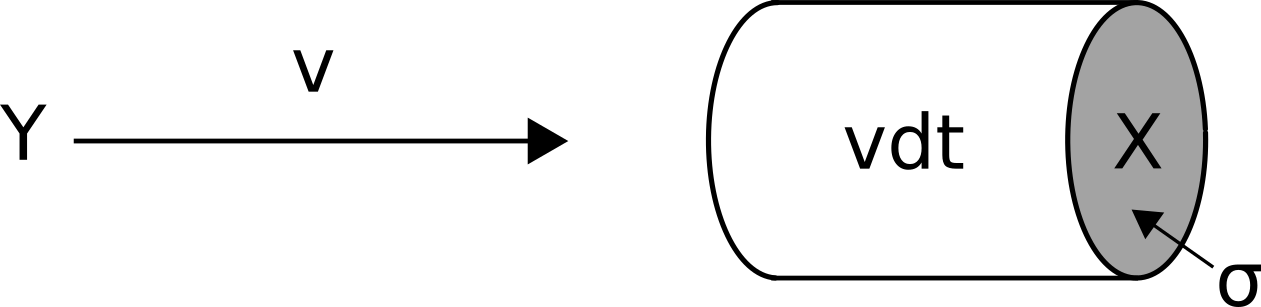
\includegraphics[width=150pt]{fig6_05}
\end{figure}

Le particelle proiettile faranno fusione quando entreranno all'interno del raggio d'azione del bersaglio.
Stiamo praticamente introducendo il concetto di  sezione d'urto.
Tutte le particelle che entreranno all'interno della zona $vdt$ avranno quindi interazione con il bersaglio ed entro un tempo $dt$ potranno raggiungere il bersaglio.
Supponendo di avere $n_Y$ particelle per unità di volume il numero di particelle che raggiungeranno il bersaglio sarà dato da
\begin{equation}
dN=n_Y \sigma vdt
\end{equation}
Si è considerato come $sigma$ l'area di interazione del bersaglio.
Si trova quindi che il numero di interazioni su di un bersaglio per unità di tempo sarà 
\begin{equation}
\frac{dN}{dt}=n_Y\sigma v
\end{equation}
Considerando ora tutti i nuclei bersaglio e generalizzando il discorso su tutte le velocità il rate diventa
\begin{equation}
Rate=n_Xn_Y<\sigma v>
\end{equation}
dove $n_X$ e $n_Y$ sono tutti i nuclei bersaglio e proiettile, e $<\sigma v>$ è una quantità media per indicare la varietà di velocità.
 
\paragraph{Analizziamo ora il termine $<\sigma v>$} Iniziamo da $\sigma$.

Classicamente la sezione d'urto è rappresentata dall'area del bersaglio
\begin{equation}
\sigma=\pi R^2
\end{equation}
\begin{figure}[h]
\centering
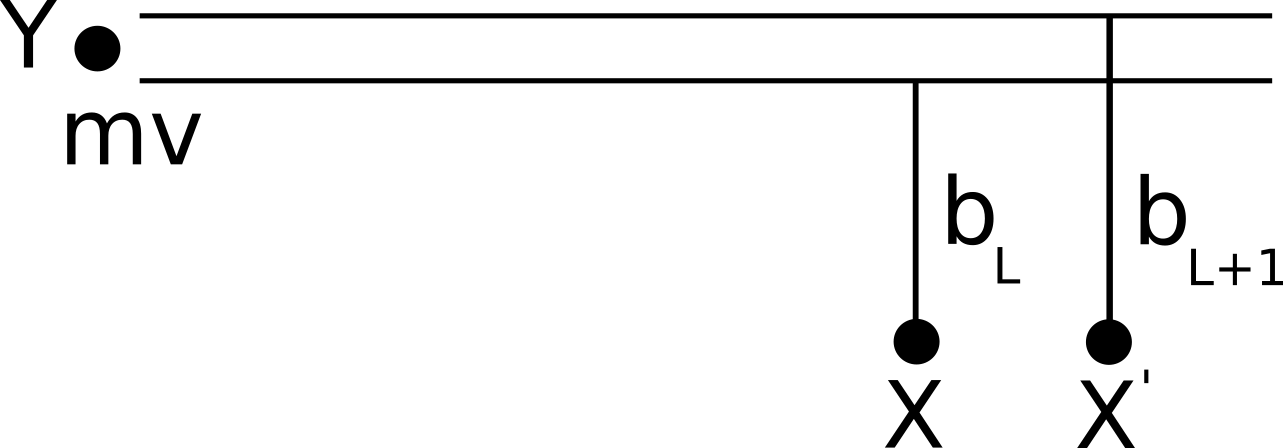
\includegraphics[width=150pt]{fig6_06}
\end{figure}

In questo caso però abbiamo a che fare con un sistema quantistico in cui le particelle che consideriamo sono anche delle onde.
Supponiamo di avere la particella $Y$ con momento angolare $m_a$, siccome siamo in un sistema quantistico questa quantità risulterà quantizzata e quindi
\begin{equation}
m_a=mvb=L\hbar
\end{equation}

Supponiamo di avere un'altra particella bersaglio, il momento angolare della seconda particella è
\begin{equation}
m_a'=mvb_{L+1}=(L+1)\hbar
\end{equation}
Supponiamo di prendere una sezione del fascio.
\begin{figure}[h]
\centering
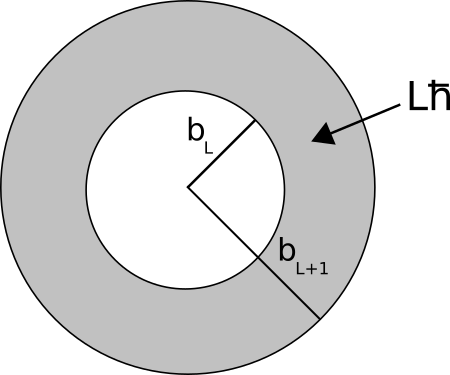
\includegraphics[width=120pt]{fig6_07}
\end{figure}

Siccome il momento angolare è quantizzato si ha che il valore del momento della corona evidenziata in figura deve corrispondere a $L\hbar$ ovvero la stessa quantità della corona interna.
L'area della corona è
\begin{equation}
A=\pi b_{L+1}^2-\pi b_L^2
\end{equation}
Ora, avendo sopra le formule dei momenti angolari quantizzati, posso calcolare le formule di $b_L$ e $b_{L+1}$ e quindi sostituirle nella formula dell'area
\begin{equation}
\begin{split}
A&=\pi \biggl[\left(\frac{(L+1)\hbar}{mv}\right)^2-\left(\frac{L\hbar}{mv}\right)^2\biggl]\\
&=\pi\frac{\hbar^2}{m^2v^2}[L^2+2L+1-L^2]\\
&=\pi \frac{\hbar^2}{m^2v^2}[2L+1]
\end{split}
\end{equation}
Per trovare la sezione d'urto finale bisogna sommare di conseguenza tutti i momenti angolari fino a che non coprirò tutto il nucleo (fino quindi al momento angolare massimo).
Come momento angolare massimo avrò
\begin{equation}
mvR=L_{max}\hbar
\end{equation}
Calcoliamo quindi la sezione d'urto totale
\begin{equation}
\begin{split}
\sigma&=\sum_{L=0}^{L_{max}}\pi \frac{\hbar^2}{m^2v^2}[2L+1]\\
&=\pi \frac{\hbar^2}{m^2v^2}[1+3+5+ ... +2L_{max}+1]\\
&=\pi \frac{\hbar^2}{m^2v^2}\left(\frac{L_{max}+1}{2}\right)+(1+2L_{max}+1)\\
&=\pi \frac{\hbar^2}{m^2v^2}(L_{max}+1)^2
\end{split}
\end{equation}
Posso quindi sostituire ad $L_{max}$ quella che trovo come dimensione del nucleo
\begin{equation}
\begin{split}
\sigma&=\pi \frac{\hbar^2}{m^2v^2}\left(\frac{mvR}{\hbar}+1\right)^2\\
&=\pi\left(\frac{\hbar}{mv}\frac{mvR}{\hbar}+\frac{\hbar}{mv}\right)\\
&=\pi\left(R+\frac{\hbar}{mv}\right)^2
\end{split}
\end{equation}
Possiamo quindi fare un paio di considerazioni. 
Il termine $\pi R^2$ all'interno della formula è il termine di interpretazione classica della sezione d'urto (vista come un'area) corrispondente alla dimensione del nucleo bersaglio.
$(\hbar/mv)^2$ rappresenta invece il termine quantistico della sezione d'urto e si può vedere che in questo caso domina la formula.
\begin{equation}
\frac{\hbar^2}{m^2v^2}=\frac{\hbar^2}{mmv^2}\frac{c^2}{c^2}=\frac{(200MeV\cdot fm)^2}{1000MeV\times 10^{-3}MeV}=200fm^2
\end{equation}
Si vede chiaramente che questa quantità è molto maggiore della del valore dato dal termine $R^2$ dato che solitamente $R=2fm$.
La sezione d'urto può quindi essere riscritta come 
\begin{equation}
\sigma=\pi^2\frac{\hbar^2}{m^2v^2}
\end{equation}
La sezione d'urto trovata riguarda solamente le particelle nella buca di potenziale ma non è stato considerato il potenziale coulombiano a di fuori della buca.
Mentre per quanto riguarda la particella nella buca di potenziale la particella è descritta dall'equazione di Shroedinger indipendente dal tempo 
\begin{equation}
\frac{d^2\psi}{dx^2}=-\frac{2m}{\hbar}(E-V_0)\psi
\end{equation}
Le cui soluzioni sono del tipo
\begin{equation}
\psi=e^{-Kx}\hspace{1cm} K=-\frac{2m}{\hbar}(E-V_0)
\end{equation}
nel caso della sezione d'urto della barriera di potenziale coulombiano, basta spostare la zona in analisi, quello che si trova è che 
\begin{equation}
P\propto |\psi|^2\propto e^{-2Kx}
\label{FF:01}
\end{equation}
in cui i valori di $E$ e $V_0$ sono i valori della barriera.

In realtà per fare un conto preciso bisognerebbe fare un integrazione con tutti i valori infinitesimi della barriera di potenziale vista come la somma di tante barriere di energia incrementale calcolate con la probabilità ~\eqref{FF:01}.
Il calcolo non viene fatto, il risultato che si ottiene alla fine è
\begin{equation}
\sigma=\frac{\pi \hbar^2}{m^2v^2}e^{\frac{-Z_1Z_2}{4\pi \varepsilon_0}\frac{2\pi}{\hbar v}}
\end{equation}
Il termine moltiplicativo iniziale è il termine senza termine coulombiano, mentre l'esponenziale rappresenta la probabilità di attraversamento della barriera.
Possiamo quindi evidenziare le dipendenze ragruppando le costanti
\begin{equation}
\sigma=\frac{C_0}{v^2}e^{-\frac{a}{v}}
\end{equation}
Per comodità si può anche esprimere la velocità in funzione dell'energia
\begin{equation}
E=\frac{1}{2}mv^2\to v=\sqrt{\frac{2E}{m}}
\end{equation}
Che restituisce la funzione della sezione d'urto desiderata
\begin{equation}
\sigma=\frac{C_0}{v^2}e^{-\frac{a}{\sqrt{E}}}
\end{equation}
Come era intuibile si vede che aumentando l'energia (e quindi la velocità) anche la sezione d'urto (ovvero la probabilità di superare la barriera) aumenta.

L'ultimo passo che manca è di tener conto della distribuzione di velocità e quindi dell'energia delle particelle.
La distribuzione maxweliana (in funzione della velocità) è
\begin{equation}
\begin{split}
N(v)&=\left(\frac{2}{\pi}\right)^{1/2}\left(\frac{m}{KT}\right)^{3/2}v^2e^{-\frac{E}{KT}}\\
&=C_0'v^2e^{-\frac{E}{b}}
\end{split}
\end{equation}
Il rate di reazione è quindi 
\begin{equation}
\begin{split}
\sigma v&=\frac{C_0}{v^2}e^{-\frac{a}{\sqrt{E}}}C_0' v^2e^{-\frac{E}{b}}\\
&=C_0 e^{-\frac{a}{\sqrt{E}}}e^{-\frac{E}{b}}
\end{split}
\end{equation}

Supponiamo di rappresentare in uno o stesso grafico la sezione d'urto, la velocità e la loro moltiplicazione, in numero di particelle particelle in funzione  dell'energia.
Quello che si vede è che le due grandezze hanno picchi opposti rispetto all'aumentare dell'energia, il che risulta nel fatto che la loro moltiplicazione possiede un picco centrale tra i due picchi detto \emph{picco di Gamov}, che corrisponde alla zona a probabilità più alta di avere fusione nucleare.
\begin{figure}[h]
\centering
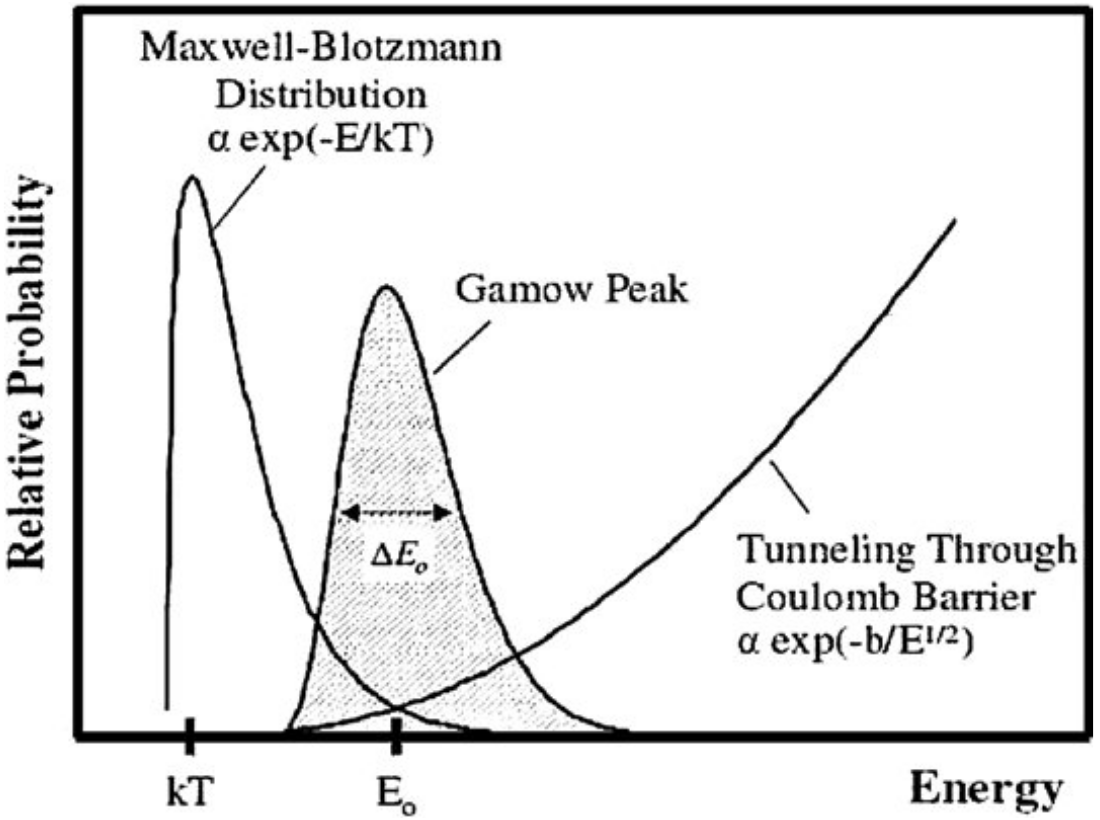
\includegraphics[width=170pt]{fig6_08}
\end{figure}

\paragraph{Fusione con il trizio}
Se fin a d'ora il processo analizzato riguardava due nuclei di deuterio, analizziamo ora una reazione del tipo
\begin{equation}
^2_1H+^3_1H\longrightarrow ^4_2He+n+Q
\end{equation}
L'energia prodotta da una reazione di questo tipo è molta
\begin{equation}
Q=17,6MeV
\end{equation}
Il problema è però che il trizio non è un isotopo così stabile in quanto decade $\beta$; 
ha una vita media di 11 anni e quindi non si può trovare in natura, è necessario quindi produrlo.
La produzione in realtà è piuttosto semplice, basta infatti ricoprire la camera di un reattore con del Litio che fare reazione con i neutroni
\begin{equation}
n+^6_3Li\longrightarrow ^3_1H+^4_2He
\end{equation}
La fusione con il trizio è preferibile a quella solamente con il deuterio perché ha un rapporto tra energia in ingresso ed energia in uscita molto più favorevole.
Si ha inoltre che per innescare e mantenere la reazione è necessario superare un certo valore di soglia dato dall'effetto di Bremsstralung che è molto presente nel plasma.
Per la reazione deuterio-trizio questo valore è di $4keV$ mentre per la reazione deuterio-deuterio è di $40KeV$.

Consideriamo ora l'energia in uscita rispetto all'energia in ingresso.
Supponiamo di avere due specie
\begin{equation}
n_x+n_y=n
\end{equation}
Per esempio uno può essere il deuterio e l'altro sia il trizio, per semplicità ne prendiamo parti uguali
\begin{equation}
n_x=n/2 \hspace{0.5cm} n_y=n/2
\end{equation}
Per mantenere il plasma una certa temperatura $D$ devo fornire in ingresso una certa energia data da
\begin{equation}
E_{ing}=\frac{3}{2}KT[2n]=3KTn
\end{equation}
L'energia in ingresso deve essere minore dell'energia in uscita altrimenti non posso sfruttare il processo per la produzione di energia.
Il rate del processo abbiamo visto che è
\begin{equation}
R=n_xn_y<\sigma v>=\frac{n^2}{4}<\sigma v>
\end{equation}
E l'energia in uscita dipenderà da questo rate appena trovato
\begin{equation}
E_{usc}=R\tau Q=\frac{n^2}{4}<\sigma v>\tau Q
\end{equation}
dove $\tau$ è detto tempo di confinamento e corrisponde al tempo in cui faccio avvenire la reazione.
La condizione necessaria per la produzione di energia è
\begin{equation}
\begin{split}
E_{usc}>E_{ing}&\to \frac{n^2}{4}<\sigma v>\tau Q > 3KTn\\
n\tau &>\frac{12KT}{<\sigma v> Q} 
\end{split}
\end{equation}
Questa condizione appena trovata viene chiamata da chi studia il plasma \emph{criterio di Lauson}.

La differenza tra la situazione deuterio-deuterio e deuterio-trizio e che ci fa preferire la seconda reazione può essere vista facendo il grafico della $n\tau$ in funzione della temperatura.
\begin{figure}[h]
\centering
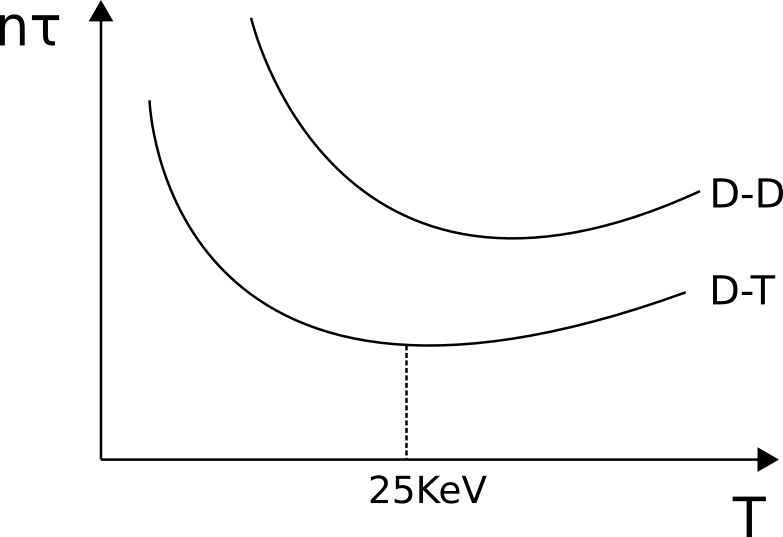
\includegraphics[width=170pt]{fig6_09}
\end{figure}

In questo grafico il criterio di Lawson è già verificata e ciò che si vuole vedere è la reazione energeticamente favorita. 
Si può notare come la reazione deuterio-trizio sia preferibile su tutti i valori di temperatura.
Il minimo che corrisponde al valore di temperatura che cerchiamo si ha per $25KeV$.
Questo corrisponde ad una temperatura di 
\begin{equation}
T=\frac{E}{K}=\frac{25KeV}{\SI{9e-5}{\frac{eV}{K}}}=\SI{3e8}{K}
\end{equation}
Che rimane più bassa della temperatura trovata inizialmente e che quindi rende già la situazione più ottimistica.

\paragraph{Confinamento magnetico}
Quello che rimane particolarmente problematico per una reazione di fusione è il confinamento.
Il plasma infatti non può venire in contatto con nessun tipo di superficie, si parla quindi di confinamento magnetico.
Si supponga di avere una particella con una certa velocità e di avere un campo magnetico.
\begin{figure}[h]
\centering
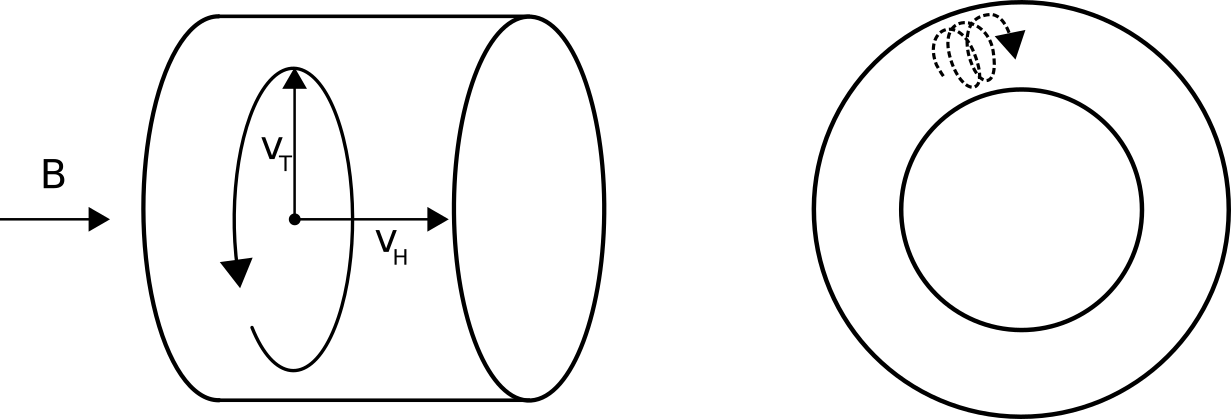
\includegraphics[width=150pt]{fig6_10}
\end{figure}

Quello che si può generare è un moto a spirale della particella, infatti la componente trasversale genera sotto campo magnetico un moto circolare che aggiunto alla velocità orizzontale diventa un moto a spirale.
Per supportare questo moto c'è quindi necessità di sfruttare una struttura simile agli acceleratori (visibile anche in figura) definita modello \emph{Tokamak}.

I problemi della fusione tecnologici rimangono comunque ancora alti (per esempio il riscaldamento del plasma) e per questo non esiste ancora un reattore funzionante. 

\paragraph{Progetti attualmente in costruzione}
Esistono dei progetti sperimentali che continuano a cercare di realizzare questo tipo di produzione energetica.
\begin{itemize}
\item Progetto \textbf{ITER} (International Thermonuclear Experimental Reactor) Realizzato in Francia con uno sforzo internazionale, sta costando miliardi e il prezzo continua ad aumentare. 
Dovebbe essere effettivamente attivo nel 2050.
\item Progetto \textbf{JET} (Joint European Thorus)
\end{itemize}
Quello che si è riusciti a raggiungere per ora è
\[
E_{out}\sim 70\% E_{in}
\] 

\paragraph{Confronto tra i processi di produzione energetica}
Si propone ora un conto di confronto tra la produzione energetica e di combustione, fissione e fusione, considerando pure i prodotti di scarto.
Il conto è a solo scopo di studio e non ha nessuna intenzione politico/propagandistica.
\begin{itemize}
\item Si comincia dallo studio della \emph{combustione di carbone}.
Iniziamo cercando si ricavare la densità energetica prodotta per unità di massa.

Ricordiamo il peso di una mole di carbone
\begin{equation}
mole_C=1,2\times10^{-3}Kg\to 1kg_C=80 mol
\end{equation} 
Per ogni reazione di combustione produciamo
\begin{equation}
1,5eV/atomo
\end{equation}
Quindi la densità energetica è
\begin{equation}
1,5\frac{eV}{atomo}\cdot 6\times10^{23}\frac{atomo}{mol}\cdot 2\times 10^{-19}\frac{J}{eV}\cdot 80\frac{mol}{kg}=10^7\frac{J}{eV}
\end{equation}
Qual'è quindi la porzione di massa che viene convertita in energia?
\begin{equation}
10^7\frac{J}{kg}\div c^2=10^{-10}\frac{energia}{massa}
\end{equation}
Significa che per esempio di una petroliera, che corrisponde a circa $100000$ tonnellate di combustibile, vengono convertiti in energia $\sim 10g$. 
Il resto è tutto residuo.

\item Si prende in considerazione la \emph{fissione dell'uranio}.

In questo caso il peso di una mole è
\begin{equation}
mole=2,4\times10^{-1}Kg\to 1kg=4mol
\end{equation}
L'energia prodotta per fissione è di 
\begin{equation}
200MeV/fissione
\end{equation}
Quindi la densità di energia dell'uranio è
\begin{equation}
2\times 10^8\frac{eV}{nucleo}\cdot 6\times10^{23}\frac{atomo}{mol}\cdot 2\times 10^{-19}\frac{J}{eV}\cdot4\frac{mol}{kg}=10^4\frac{J}{kg}
\end{equation}
Il che significa che la massa convertita corrisponde a
\begin{equation}
10^{-3}\frac{energia}{massa}
\end{equation}
Il che vuol dire che $10g$ di massa convertita corrispondono a $10kg$ di materiale sfruttato, il resto sono scorie, purtroppo altamente radioattive.

\item Passiamo infine alla \emph{fusione nucleare}.

Una mole di materiale corrisponde a 
\begin{equation}
mole=2\times10^{-3}kg\to 1kg=500mol
\end{equation}
Con un'energia per fusione pari a 
\begin{equation}
17,6MeV/fusione
\end{equation}
La densità energetica è
\begin{equation}
1,8\times 10^7\frac{eV}{fusione}\cdot 6\times10^{23}\frac{atomo}{mol}\cdot 2\times 10^{-19}\frac{J}{eV}\cdot 250\frac{mol}{kg}=5\times 10^14\frac{J}{kg}
\end{equation}
(vanno considerate metà moli perché la fusione riguarda due nuclei al posto che uno).

La conversione sarà quindi di 
\begin{equation}
5\times 10^{-2}\frac{energia}{massa}
\end{equation}
Ciò vuol dire che per convertire $10g$ di materiale necessito di $5kg$ di deuterio/trizio, il resto sarà residuo, ma in questo caso di $He$ che non è radioattivo (e dal punto di vista dell'inquinamento prevede quantità molto più limitate di emissioni rispetto al carbone).
\end{itemize}